\chapter{Hardware}

I det følgende afsnit beskrives systemet hardware vha. SysML diagrammer. 
Indledningsvis bruges bdd'er til at identificere og beskrive systemets blokke. Senere i afsnittet vises blokkenes interne og eksterne forbindelser med ibd'er.

\section{Block definition diagram}
I det overordnede bdd nedenfor vises hvilke blokke systemet består af samt hvilke parts blokkene har. Det ses at systemet helt overordnet set kun består af de to blokke - \textit{Webapplication} og \textit{Drone}. 

\begin{figure}[H]
\centering
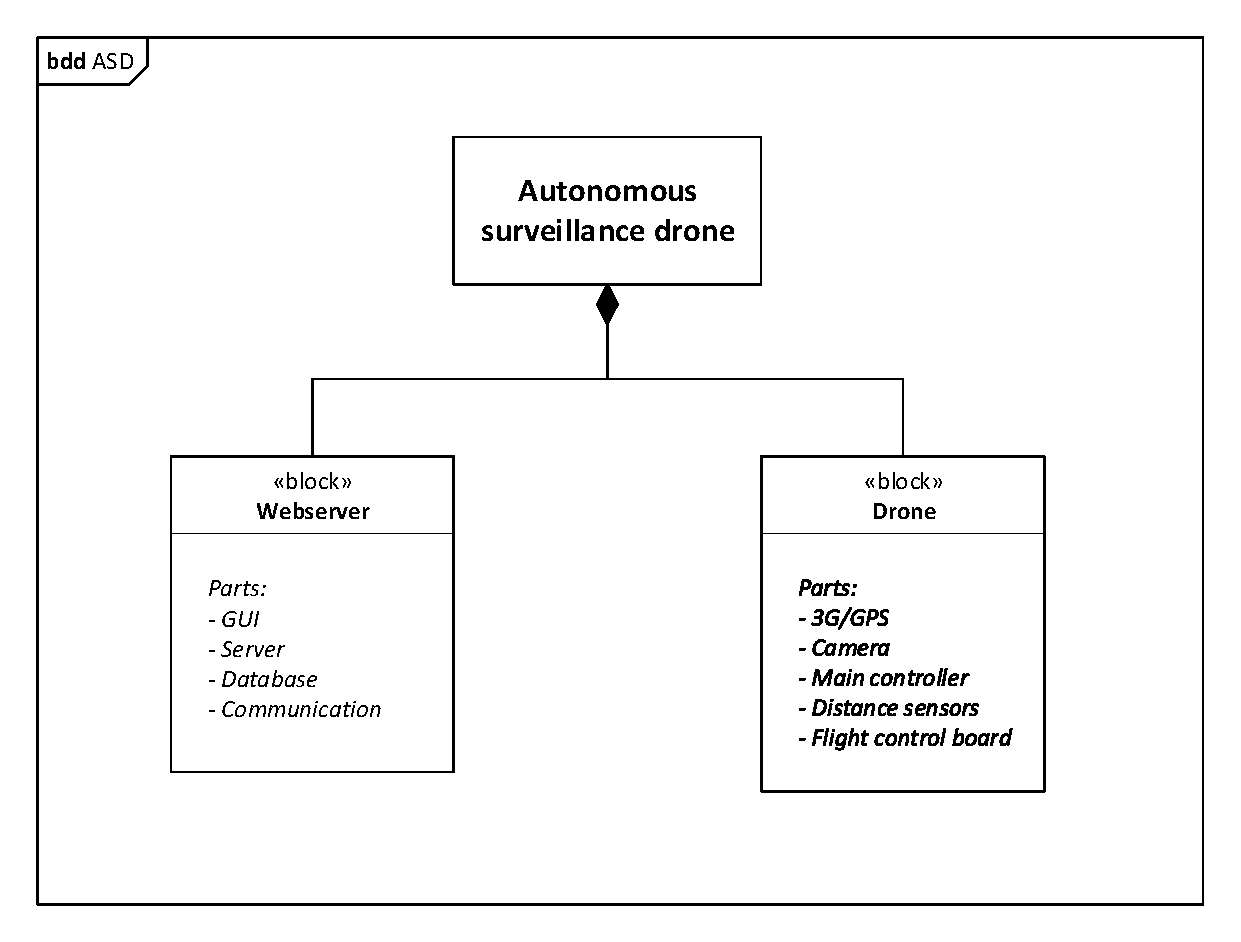
\includegraphics[width=1\textwidth]{Billeder/BDD/bdd_overordnet.pdf}
\caption{Overordnet bdd}
\label{fig:bdd_overordnet}
\end{figure}

\newpage
\subsection{Udvidet - Block definition diagram}
Figur \ref{fig:bdd_drone} går mere i dybden med drone blokken. På denne figur er drone blokken blevet åbnet op, og det vises nu hvilke blokke dronen er bygget af. 

\begin{figure}[H]
\centering
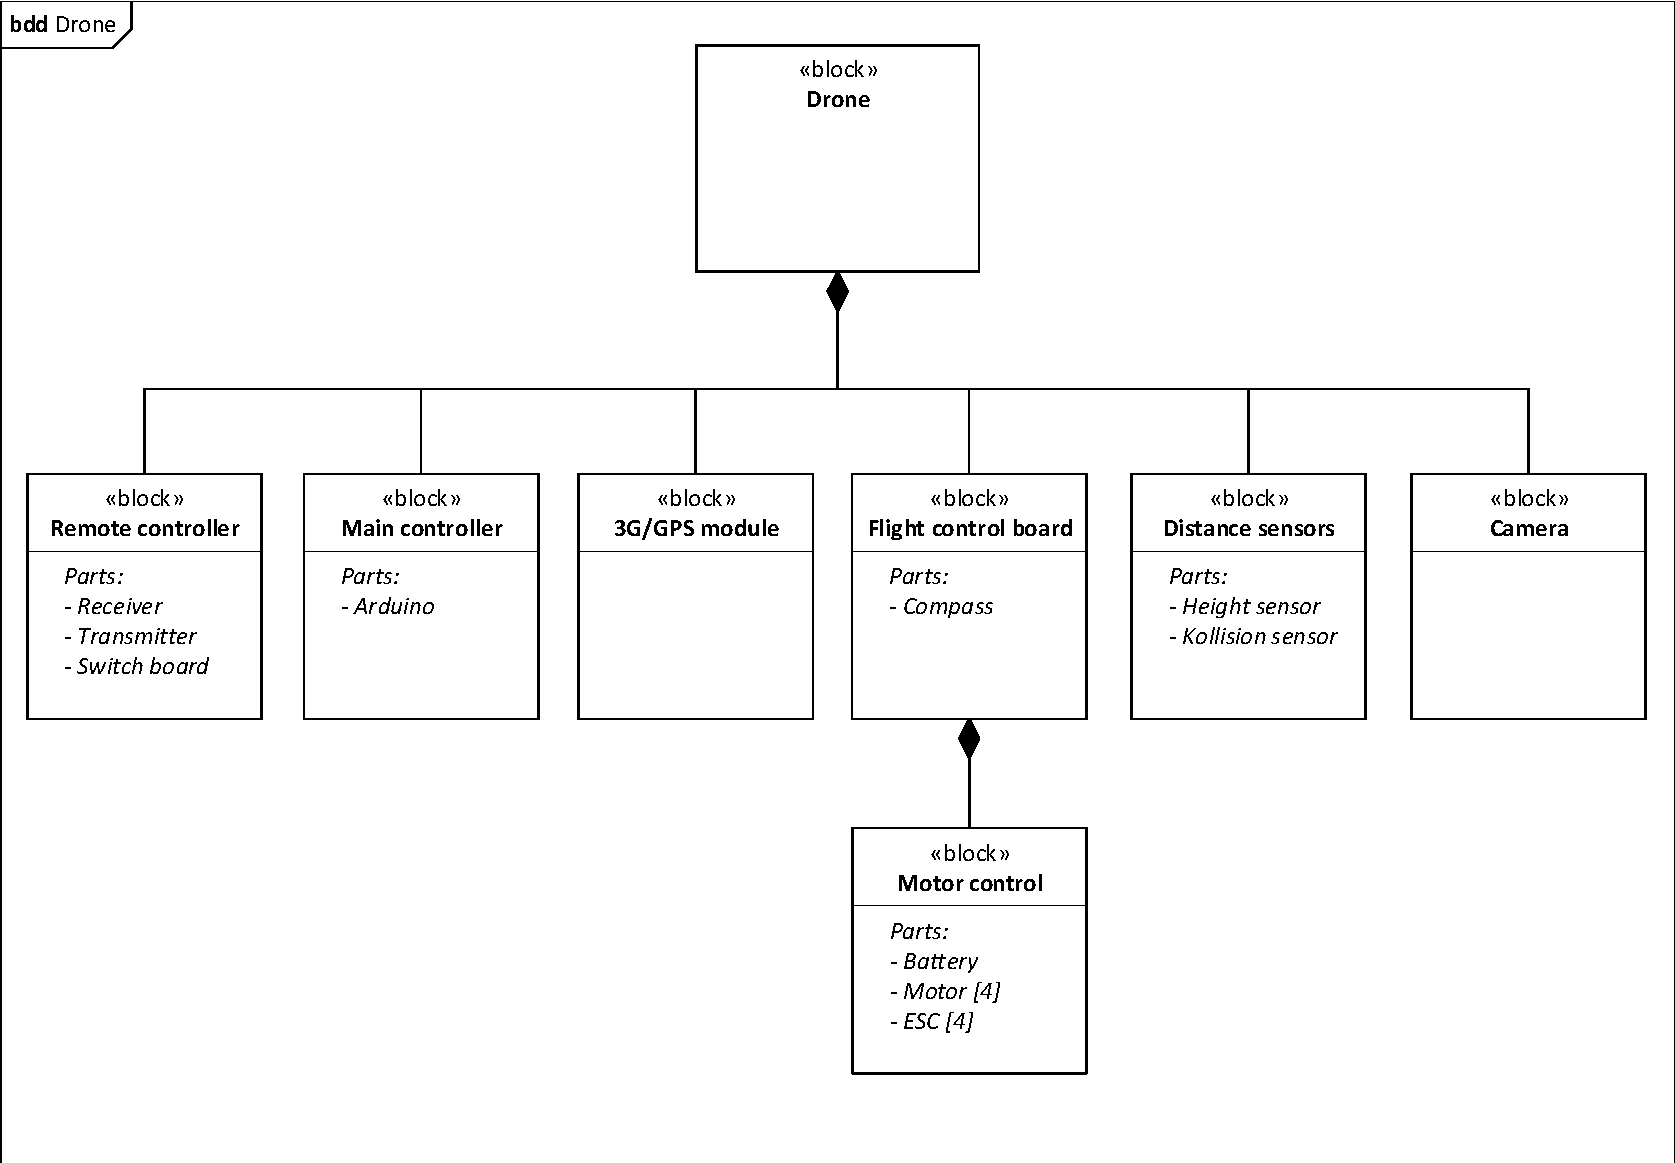
\includegraphics[width=1\textwidth]{Billeder/BDD/bdd_drone.pdf}
\caption{Drone - bdd}
\label{fig:bdd_drone}
\end{figure}

\newpage

\subsection{Blokbeskrivelse}

\textbf{Webapplikation}\\
Denne blok dækker over server, GUI, database og kommunikation. Via GUI tilgår bruger webapplikationens server, herfra er det muligt for bruger at opsætte ny eller undersøger en tidligere flyvning. Webapplikationen kommunikerer med dronen og gemmer vigtig information i databasen.

\textbf{Main controller}\\
Main controlleren fungerer som dronens hjerne. Ud fra kommunikation med webapplikation og input fra de forskellige sensorer styrer main controlleren dronens motorer. Skal dronen fx. flyve højere udsendes PWM signaler fra main controller til flight control board, som sørger for motorerne øger rotationshastigheden. 

\textbf{Flight control board}\\
Flight control boardet indholder styring software, derunder PID regulering. Boardet har indbygget kompas, gyroskop, accelerometer og barometer, disse bruges under flyvning. Flight control boardets vigtigste opgave er at viderebringe control signaler fra main controller til ESC'er som åbner/lukker for forsyning til motorer. 

\textbf{3G/GPS}\\
3G/GPS blokken har to funktioner i systemet. For det første er 3G/GPS blokken ansvarlig for opdatering af dronens GPS position. Desuden fungerer blokken som kommunikationslag mellem webapplikation og main controller. Al information der udvekles mellem webapplikation og drone går gennem 3G/GPS modulet. Som navnet indikerer, kan modulet tilkobles 3G mobilnetværk.  

\textbf{Afstandssensorer}\\
Afstandssensorerne bruges både til måling af flyvehøjde og til anti kollision. Sensorerne fungerer \textit{aktiveres} af main controlleren når ny højdemåling eller tjek af forhindring skal foretages. Sensorerne bruger 40 kHz signaler til at måle distancen til jorden eller eventuelle forhindringer.

\textbf{Kamera}\\
Når dronen er i rette position modtager kameraet besked og tager et billede. Billedet tages og sendes videre i systemet til godkendelse - Der tages nyt eller flere nye billeder, hvis det første billede ikke godkendes.

\textbf{Motor control}\\
Denne blok består af ESC, batteri og motorer. Blokken styres med PWM signaler af flight control boardet.
